% +--------------------------------------------------------------------+
% | Sample Chapter
% |
% | This file provides examples of how to
% | - insert a figure with a caption
% | - construct a table with a caption
% | - create subsections within the chapter
% | - insert a reference to a Figure or Table
% | - make a citation
% +--------------------------------------------------------------------+

\cleardoublepage

% +--------------------------------------------------------------------+
% | Replace "Chapter Title" below with the title of your chapter.  LaTeX
% | will automatically number the chapters.
% +--------------------------------------------------------------------+

\chapter{Introducción}
%\label{ch:chapter1}
\label{makereference}

Entre los años 2008 y 2009 se comenzó a usar el concepto Internet de las cosas (abreviado IoT) como una apuesta hacia el futuro, cuyo objetivo era interconectar dispositivos digitales a internet.

Esto ya es una realidad, con mayor frecuencia encontramos nuevos dispositivos capaces de conectarse a internet, permitiendo al usuario su manejo desde cualquier parte del mundo. Con ello se abre camino a nuevas oportunidades haciendo la vida más cómoda al usuario y proporcionándole mayor seguridad y control.

Según empresas del sector tecnológico, en 2016 se espera que haya más de 6.000 millones de dispositivos basados en este concepto.

El concepto del internet de las cosas agrupa múltiples capacidades, algunas de ellas han sido utilizadas en el proyecto, estas se nombran a continuación:

\textbf{Comunicación y cooperación:} Dispositivos capaces de conectarse a la red de internet y entre ellos, intercambiando datos y comunicándose con servidores.

\textbf{Direccionamiento:} Los objetos serán localizables y configurables desde cualquier lugar de la red de internet.

\textbf{Identificación:} Los objetos se identificarán en la red por medio de tecnologías como RFID (Radio Frecuency Identification), códigos de barras ópticos, NFC (Near Field Communication) y otras muchas formas.

\textbf{Localización:} Se podrá saber la ubicación física del dispositivo en cualquier momento.

El proyecto nace con el objetivo de emprender en esta tecnología, para ello se quiere conectar entre sí un sensor de acelerometría y un microprocesador para recibir y procesar sus datos. Dicho microprocesador debe estar provisto de Bluetooth de Bajo Consumo (en inglés, Bluetooth Low Energy o BLE) para poder enviar los datos vía Bluetooth a una aplicación móvil desarrollada en Android creada por los alumnos.

Existe una amplia variedad de dispositivos de bajo coste que podrían considerarse, ya que el mercado de los microprocesadores de bajo consumo está ahora en expansión y hay gran oferta de estos dispositivos, con entornos de desarrollo que ofrecen distintas alternativas y que previsiblemente irán reduciéndose en los próximos años cuando predomine una tecnología que se imponga a las demás.

Unas de las  empresas más especializadas en este tipo de tecnologías y que resaltan en este mercado son \textbf{Nordic Semiconductor, Cypress Semiconductor, Texas Instruments (TI), Cambridge Silicon Radio (CSR)} y \textbf{Dialog Semiconductor}.

Destacamos 2 empresas que nos han ofrecido mejores soluciones de microprocesadores de bajo consumo según las necesidades del proyecto:

\textbf{Nordic} está a la vanguardia de la revolución inalámbrica y son especialistas en Radiofrecuencia de consumo ultra bajo (ULP) redefiniendo nuevos procesadores por su bajo consumo, precios competitivos y aumentando la potencia de estos.
Esta empresa de semiconductores integra procesadores basados en la arquitectura ARM de 32 y 64 bits que predominan en el mercado de la electrónica. Son procesadores relativamente simples siendo ideales para aplicaciones de bajo consumo y tiene un precio económico. 

\textbf{Cypress} es una empresa especializada en ofrecer soluciones de alta calidad para sistemas integrados en el sector aeroespacial, automoción, industria, redes, telecomunicaciones y electrónica de consumo, entre otros campos. Cubre una amplia gama de productos entre los cuales destacan los microprocesadores, memorias,  sistemas programables en chips , lo que denominan (en inglés Programable System on Chip o PSOC), controladores táctiles capacitivos y controladores inalámbricos Bluetooth de bajo consumo

\section{Entornos de desarrollo}
\label{makereference1.1}

Con los dispositivos de bajo consumo nacen también multitud de entornos de desarrollo específicos para desarrollar todo su potencial, lo que dificulta la exploración de hardware, pues es necesario trabajar con un nuevo entorno cada vez. 

mbed, creada por la empresa ARM, es una plataforma de desarrollo \textit{online} que intenta hacer frente a esta variedad de entornos facilitando el desarrollo de prototipos de sistemas basados en microprocesadores.

Esta plataforma se creó para promover el Internet de las Cosas (IoT) y desarrollar proyectos mediante herramientas de construcción de hardware y software que aceleren el desarrollo de dispositivos basados en ARM.

Su enfoque está basado en la \textit{nube} y permite codificar, añadir librerías y compilar desde un navegador web. La ventaja de programar desde cualquier navegador es que permite tener accesibilidad desde cualquier punto del mundo sólo con conexión a internet. Durante el Capítulo~\ref{makereference4} se explicará con más detalle este entorno y cómo nos ha ayudado a llevar a cabo este proyecto.

Todo lo anterior hace de la compatibilidad con mbed una característica atractiva a la hora de elegir un dispositivo para llevar a cabo nuestro proyecto, lo que nos ha ayudado a elegir la placa de desarrollo nRF51-DK de Nordic.

\section{Bluetooth Smart: Bluetooth de bajo consumo}
\label{makereference1.2}

Uno de los rasgos fundamentales de IoT es la conectividad. Para lograrla tenemos a nuestra disposición una gran variedad de tecnologías inalámbricas, entre ellas \textit{zygbee}, \textit{narrow-band} o \textit{WiFi}; pero la que sin duda alguna ofrece el menor consumo de energía posible es \textit{Bluetooth Low Energy} (BLE, también denominado \textit{Bluetooth Smart}). 
Esta tecnología nace del Bluetooth clásico, pero marca su propio camino al sacrificar ancho de banda y períodos de envío continuados para lograr la meta de ser muy eficiente energéticamente, lo que lo hace perfecto para dispositivos que necesitan funcionar con una batería pequeña durante largos períodos. El hecho de ser parte de Bluetooth y poderse complementar con él hace que actualmente esté presente en todos los teléfonos móviles del mercado. A esto ayuda que grandes empresas del mundo de la tecnología y las telecomunicaciones respalden BLE.

En el Capítulo~\ref{makereference2} hablaremos de cómo se estructura e implementa Bluetooth Low Energy. 

\section{Especificación del objetivo del proyecto}
\label{makereference1.3}

El objetivo de este proyecto consiste en medir el esfuerzo realizado por un ciclista durante un trayecto. Esto se consigue combinando los valores proporcionados por un acelerómetro y los datos de posicionamiento por GPS para poder elaborar un mapa del trayecto en el que se indiquen las zonas que, por pendiente, estado del terreno, etc. supusieron un mayor esfuerzo. Además se ofrecerá más información que pueda ser calculada con estos datos, como la velocidad media o la distancia total recorrida, por ejemplo.

Para la comodidad del usuario, toda la información de la ruta se recogerá en su dispositivo móvil, del que se obtendrán los datos de localización y que se conectará a través de Bluetooth Smart con el sensor de acelerometría. De este modo, con un simple gesto podrá visualizar fácilmente los datos más relevantes.

\begin{figure}[h]%t=top, b=bottom, h=here
	\centering
    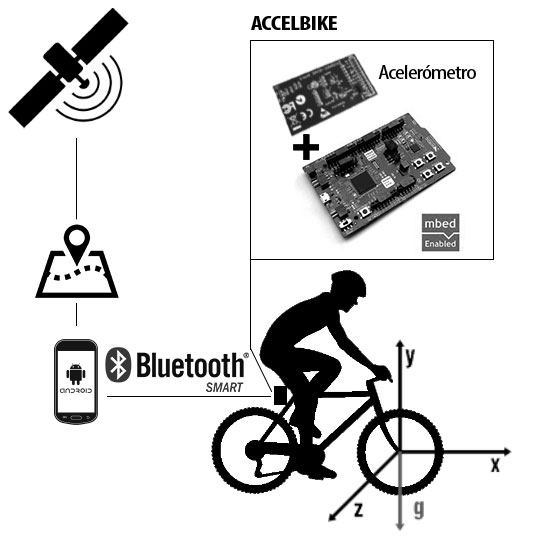
\includegraphics[scale=0.5]{figures/esquema_accelbike.jpg}
    \caption[Esquema del funcionamiento del proyecto]{Esquema del funcionamiento del proyecto. El dispositivo móvil recoge datos tanto de la localización como de un sensor de acelerometría.}
   	\label{figuraEsquemaAccelbike}
\end{figure}

\newpage % Esto esta aqui para que la imagen anterior no se meta dentro de las contribuciones

\section{Contribuciones Personales}
\label{makereference1.4}

\subsection{Rodrigo Claudio Miguez Rein}

La tarea principal que he realizado durante este proyecto es la de la programación de la placa nRF51-DK de Nordic para configurar la recepción de las muestras de acelerometría utilizando el bus de datos I2C y el envío de éstas por medio de la tecnología Bluetooth Low Energy. Además he realizado la parte BLE de la aplicación Android.

En cuanto elegimos este proyecto, empecé a recopilar información junto con mis compañeros sobre las distintas soluciones \textit{System on Chip} con Bluetooth Smart integrado disponibles en el mercado. Para ello me informé sobre las tecnologías disponibles para realizar la conexión con un acelerómetro y sobre qué características necesitábamos en términos de procesamiento, memoria RAM y flash.

Durante este periodo también comencé a investigar sobre el funcionamiento y las características de Bluetooth Low Energy, buscando material de referencia para aprender todo lo posible sobre ésta.\\

Una vez escogimos dos placas de desarrollo, el kit CY8CKIT-042-BLE~\cite{CypressDatasheet} de la empresa Cypress Semiconductor y el modelo nRF51-DK de Nordic Semiconductor, comenzamos la fase de pruebas para familiarizarnos con las tecnologías que íbamos a usar. En mi caso, realicé las pruebas con la placa de Cypress. Para ello busqué tutoriales en la página web oficial de la empresa~\cite{CypressTutorials} y encontré un repositorio en GitHub con 100 proyectos de ejemplo~\cite{100Projects} que me ayudaron en gran medida para entender la programación del kit y los métodos para utilizar Bluetooth Low Energy y para realizar la comunicación con otros dispositivos. Descargué la aplicación móvil \textit{CySmart}, que permite probar los códigos de ejemplo con una interfaz limpia y clara, que además ofrece su código fuente, lo que me sirvió para comprobar cómo se realiza el enlace por Bluetooth Low Energy en el lado de Android.

Entre los ejemplos disponibles para esta placa se encuentran: un sistema de alerta, que consiste en el envío de una señal al dispositivo para apagar o encender un LED y para hacer que parpadee, una aplicación de sensor de proximidad, que aprovecha un circuito integrado en la placa de desarrollo diseñado para este fin, enviando el valor recogido por el sensor al móvil, donde, con la aplicación CySmart mencionada anteriormente, se puede visualizar como una escala.

Durante la fase de pruebas realicé el código que permitía al CY8CKIT-042-BLE leer por SPI los datos recogidos de un circuito, consistente en un conversor analógico-digital contectado a una fotoresistencia, y enviarlos por Bluetooth Low Energy a una aplicación de prueba realizada en Android. Seguidamente comencé con las pruebas para recibir por I2C los datos del acelerómetro. Estas pruebas se detallarán más adelante en esta memoria.

Cuando elegimos la placa de Nordic, escogí continuar la parte del proyecto que se centraba en la programación de ésta, ya que me había resultado muy interesante la experiencia con el kit de Cypress. Realicé la conexión por I2C de Xtrinsic Sense-Board, una placa que contiene un chip de acelerometría. Para ello busqué su \textit{datasheet}~\cite{DatasheetAcc} para saber qué pines utilizaba, de qué manera recolectaba las muestras y cómo había que realizar la comunicación entre nRF51-DK y este periférico para lograr una transmisión correcta de los datos. Una vez pude comprobar que se recibía la información de acelerometría, elaboré un sistema para filtrar el ruido presente en las muestras y realicé la configuración de la placa de Nordic para que las transmitiera utilizando Bluetooth Low Energy.

En la parte de la aplicación Android, ayudé con el diseño de las clases que se iban a utilizar elaborando diagramas, y proporcioné \textit{feedback} a mis compañeros para hacerles saber en qué formato se iba a mandar la información por Bluetooth para que pudieran configurar en consecuencia la lectura de éstos en el móvil.

\subsection{David Muñoz Lorenzo}

Mi labor en el proyecto en su fase inicial, como la de mis compañeros, fue analizar en detalle los componentes que íbamos a utilizar para la elaboración del sistema de acelerometría. En primer lugar debíamos encontrar en internet los microprocesadores Bluetooth Low Energy que dieran solución al objetivo del proyecto.
Se planteó hacer la búsqueda eligiendo los componentes más económicos y con las prestaciones suficientes para realizar el proyecto, siendo elaborado como producto final. Analicé en profundidad microprocesadores de diferentes marcas y características que debían ser compatibles con las conexiones SPI e I2C.

Se decidió elegir 2 placas de desarrollo, nRF51-DK de Nordic Semiconductor y CY8CKIT-042-BLE de la empresa Cypress Semiconductor, que nos ofrecían dichas conexiones, así como Bluetooth de bajo consumo y múltiples periféricos, lo cual eran soluciones más que suficientes para empezar.

Para realizar la primera prueba con la placa de Nordic, tuvimos que crear un sencillo circuito para recoger datos desde una fotoresistencia, y convertir la señal que recibíamos en una señal digital para poder enviársela a la placa de desarrollo.

Participé en la creación de dicho circuito así como en las pruebas de desarrollo para realizar la conexión por SPI y recibir los datos que transmitía la fotoresistencia.

Tuvimos que familiarizarnos con el entorno de desarrollo llamado mbed que utilizaba la placa de Nordic. En su repositorio~\cite{repoMbed} pudimos probar ejemplos de conexiones SPI que adaptamos a la placa utilizada, mirando en su ficha técnica~\cite{NordicDatasheet} la correcta conexión de sus pines.

La manera de interactuar con la fotoresistencia a través de la placa fue activar los LEDs que esta contiene, alternándolos según su valor de entrada. De esta forma verificamos que el paso de datos funcionaba correctamente.

La siguiente prueba de conexión fue a través de I2C, tuvimos que investigar y documentarnos bien sobre este bus de datos. Se cambió el circuito por un acelerómetro que conectamos por I2C a la placa de desarrollo.

En este punto fue necesario investigar la forma de crear una aplicación en Android, de tal forma que esta pudiera conectarse por Bluetooth Low Energy a la placa nRF51-DK de Nordic y visualizar los datos recibidos. Para realizar la prueba de conexión por Bluetooth encontramos en el repositorio de mbed algunos ejemplos que nos ayudaron a poder implementar el módulo BLE.

Realicé una maqueta visual (\textit{mockup}) de cada vista para poder tener un primer diseño de la aplicación en el que fijarnos.
Participé en la creación de la aplicación en Android desarrollando la interfaz de usuario y su estructura. Estructuré la aplicación con un tipo de componente de Android llamado Fragment que se usa mucho en la actualidad y que sirve para separar las diferentes vistas para que puedan tener su propia lógica de manera independiente. Quise darle un aspecto y usabilidad propios de las nuevas aplicaciones de última generación utilizando componentes gráficos de Material design de Google~\cite{MaterialDesignGoogle}. De esta forma nuestra aplicación se beneficia de los últimos avances visuales asegurando una óptima experiencia de usuario. 

Realicé pruebas obteniendo los datos del GPS del móvil y realizando la petición a través de un servicio interno. Utilicé la interfaz LocationListener que nos  permite conectarnos con los servicios de ubicación del dispositivo móvil. Pude obtener la latitud y longitud de la ubicación en la que nos encontramos y a través de unos parámetros podemos cambiar la distancia ( metros ) que actualiza el GPS así como configurar la frecuencia de muestreo ( milisegundos ) de las coordenadas. Posteriormente se utilizó un hilo para poder recibir los datos del acelerómetro aunque la aplicación estuviera activa en segundo plano.

Debíamos mostrar el circuito recorrido por un ciclista desde que se pone en marcha hasta que finaliza su recorrido. Para visualizar el mapa utilizamos la API de Google Maps~\cite{APIGoogleMaps}. Para poder utilizar sus funcionalidades principales tuve que registrarme en la API de Google Maps, incorporamos al proyecto una clave única que para tener acceso a las funcionalidades de su servidor. Activé los permisos necesarios para obtener el mapa de Google y sus configuraciones necesarias para ajustarlo a nuestra aplicación. Utilizando la clase polilíneas de Google pude crear las líneas sobre el mapa, se pudo visualizar con éxito en la vista Actividades.

\subsection{Alexis Vizcaya Hervella}

Mi contribución al proyecto ha sido principalmente la de estructurar el código de la aplicación Android, centrándome en la parte del análisis de los datos y los cálculos realizados con ellos, así como de la lectura y escritura de los mismos.  

En el primer cuatrimestre iniciamos en conjunto una investigación general haciendo un análisis de los dispositivos que incorporaran la tecnología Bluetooth Low Energy (BLE) disponibles en el mercado que se ajustaran a los requisitos del proyecto, comparamos precios, características, etc. y finalmente escogimos las placas de desarrollo de Cypress (PSoC 4 BLE) y Nordic (nRF51-DK). Una vez elegidas las placas, investigué los buses de datos I2C y SPI puesto que estas eran las tecnologías disponibles en ambas para la comunicación con un acelerómetro. Además inicie el proceso de familiarización con los entornos de desarrollo.

En una primera etapa realice ejemplos con la placa de Cypress en su entorno de desarrollo (PSoC Creator) ya que descubrimos la existencia de un repositorio en GitHub que contenía 100 proyectos de ejemplo, probé con varios ejemplos para comprender la forma de diseñar pequeños programas en dicha placa, además disponía de una app para el teléfono móvil para poder conectar con la placa y así poder realizar estos ejemplos. 

Con la placa de Nordic ocurrió algo similar, con su entorno de desarrollo mbed, cuyo repositorio oficial contiene multitud de ejemplos, con los que empecé a investigar acerca del funcionamiento de esta. Como por ejemplo uno con el que empecé a establecer la conexión Bluetooth con el móvil, consistente en detectar la pulsación de un botón en la placa y mandar la información del estado de éste a una app.

Una vez finalizada esta etapa de aprendizaje hicimos pruebas de conexión entre la placas y un circuito MCP mediante SPI. El circuito constaba de una fotorresistencia conectada a un ADC con la que comprobamos que al cambiar la luminosidad que recibÍa la resistencia los datos que obteníamos en la placa variaban. El siguiente paso fue conectar un acelerómetro mediante I2C a la placa de Nordic, pudimos comprobar que los datos se recibían correctamente a través de los LEDs de los que disponía la placa, y una vez comprobado el correcto funcionamiento, nos dispusimos a realizar la conexión mediante BLE entre una pequeña app y la nRF51-DK. 

Una vez decidida la placa con la que íbamos a afrontar el proyecto, comenzamos con el diseño de la aplicación Android, forme parte del diseño de la estructura mediante un patrón Modelo Vista Controlador (MVC) y en el desarrollo del menú principal de la aplicación. 

A partir de aquí me centré en la parte de lectura y escritura de la información recibida, decidiendo cómo se iban a llevar a cabo estos procesos. 
Sobre la lectura desarrolle el proceso por el cual se finaliza una sesión y se traslada toda la información a un vista con un mapa de Google Maps con la ruta dibujada en forma de polilínea y una serie de campos para mostrar la información procesada. 
Sobre la escritura, elegí la forma de guardar los datos en la memoria externa del teléfono móvil como se describirá en esta memoria.   

Para recoger los datos de las diferentes fuentes, programé la estructura de hilos que se utiliza en la aplicación, ya que teníamos que tener un control para asignar diferentes periodos de tiempo, debido a que por ejemplo no es necesario recopilar la información del GPS tan a menudo como la del acelerómetro.

%\begin{figure}[htb]%t=top, b=bottom, h=here
%
%    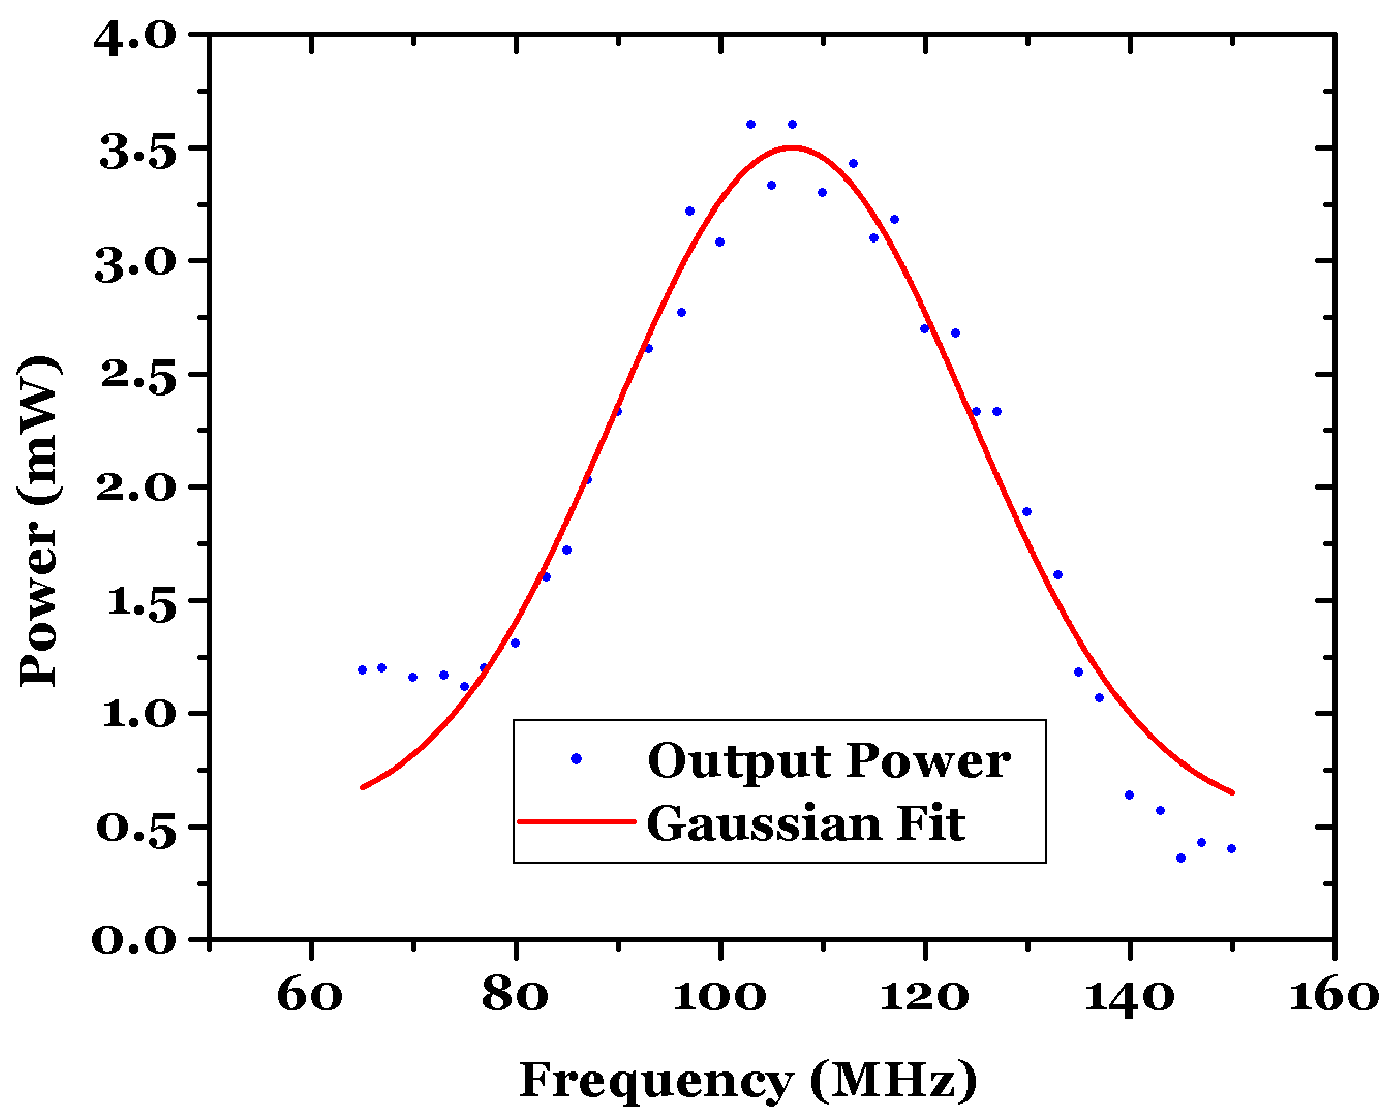
\includegraphics[height=2.5in]{figures/graph.png}
%
%    \caption[Optional: Short caption to appear in List of
%    Figures]{Full caption to appear below the Figure}
%
%   \label{figure1}
%\end{figure}

% +--------------------------------------------------------------------+
% |To create cross-references to figures, tables and segments
% |of text, LaTeX provides the following commands:
% |   \label{marker}
% |   \ref{marker}
% |   \pageref{marker}
% | where {marker} is a unique identifier.
% |
% | In the line above, we use \label{figure1} to mark a location
% | we wish to refer to later.  LATEX replaces \ref by the number of
% | the chapter, section, subsection, figure, or table after which the
% | corresponding \label command was issued. \pageref prints the page
% | number of the page where the \label command occurred.
% |
% +--------------------------------------------------------------------+

%Here is an example of a Table:

%\begin{table}

% +--------------------------------------------------------------------+
% | We include the command \begin{center} to center the table
% | horizontally on the page.  Note use of the command \end{center}
% | to turn off centering after the table is defined.
% +--------------------------------------------------------------------+
%    \begin{center}

% +--------------------------------------------------------------------+
% | The table is created with this command
% |
% | \begin{tabular}[pos]{table spec}
% |
% | The "pos" argument specifies the vertical position of the table relative to
% | the baseline of the surrounding text.  Use t, b, or c to specify alignment
% | at the top, bottom, or center.
% |
% | The "table spec" command defines the format of the table
% |   l for a column of left-aligned text
% |   r for a column of right-aligned text
% |   c for centered text
% |   p{width} for a column containing justified text with line breaks
% |   | for a vertical line
% +--------------------------------------------------------------------+

%    \begin{tabular}[c]{|c|c|c|}
%        \hline
%        Column 1 Heading & Column 2 Heading & Column 3 Heading \\
%        \hline
%        Col 1 Row 1 & Col 2 Row 1 & Col 3 Row 1\\
%        Col 1 Row 2 & Col 2 Row 2 & Col 3 Row 2\\
%        Col 1 Row 3 & Col 2 Row 3 & Col 3 Row 3\\
%        \hline
%    \end{tabular}
%    \caption{Caption to appear below the table}
%    \label{table1}
%   \end{center}
%\end{table}

% +--------------------------------------------------------------------+
% | Replace \section headings below with the title of your
% | subsections.  LaTeX will automatically number the subsections 1.1,
% | 1.2, 1.3, etc.
% +--------------------------------------------------------------------+

%In this paragraph, we want to refer to Fig.~\ref{figure1}
%mentioned at the beginning of this chapter.  We also refer to the
%Table~\ref{table1}.

%\section{Making a Reference to a Chapter Subsection}
%\label{makereference1.2}

%In this section, we refer back to text mentioned in
%Section~\ref{makereference1.1} on page~\pageref{makereference1.1}.

%\section{Making a Citation}
%\label{makereference1.3}

%Here's an example of a citation to a single
%work.~\citet{CT:Weiner:1999} It's also possible to make multiple
%citations.~\citet{CT:Phillips:1985, ARP:Loy:1974}
